\section{Microbenchmarks}
\label{sec:micro}

We first evaluate the effectiveness of Presto over a series of microbenchmarks. Using 
canonical topologies, we investigate (i) Presto's effectiveness in preventing the small segment
flooding problem and reordering, (ii) Presto's CPU overhead, (iii) Presto's ability to scale
to multiple paths, (iv) Presto's ability to handle congestion, (v) comparison to flowlet
switching, and (vi) comparison to local, per-hop load balancing.

%%%%%micro test - scalability and congestion test topology
\begin{figure}[t]
        \centering
	\begin{subfigure}[b]{0.225\textwidth}
        	\centering
  		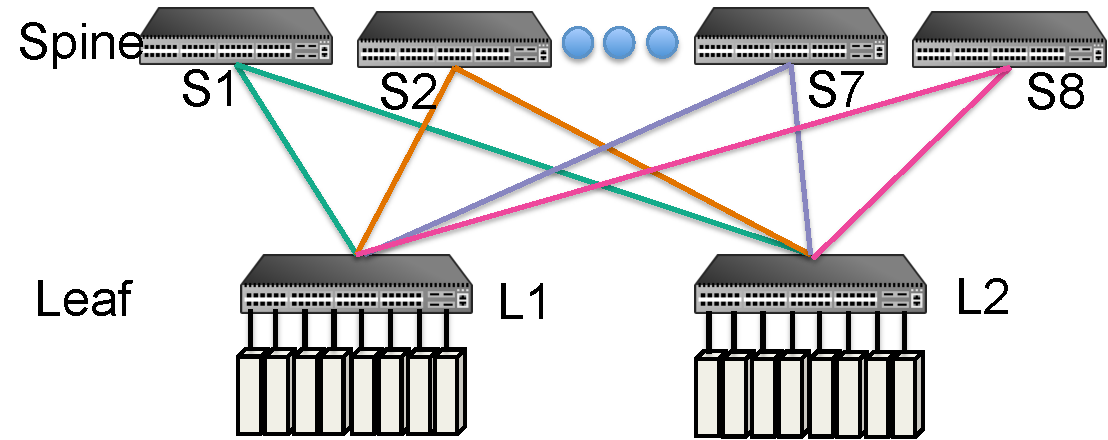
\includegraphics[width=\textwidth]{./figures/micro_test_topology/micro_scalabilitytest_topology_refined.pdf}
        	\caption{}
		\label{micro_scalability_topology}
	\end{subfigure}
	\begin{subfigure}[b]{0.225\textwidth}
                \centering
		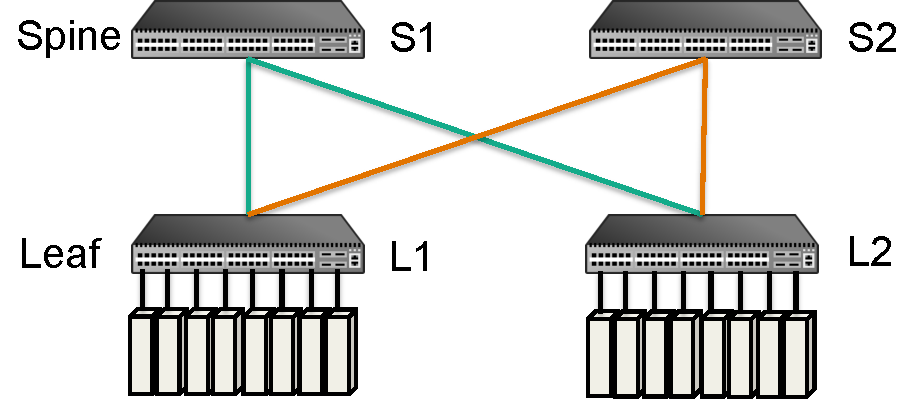
\includegraphics[width=\textwidth]{./figures/micro_test_topology/micro_congestiontest_topology_refined.pdf}
        	\caption{}
		\label{micro_congestion_topology}
	\end{subfigure}
	\caption{(a) Scalability benchmark and (b) Oversubscription benchmark topology.}
	\label{micro_topology}
\end{figure}

%%%%%gro effectiveness shows
\begin{figure}[t]
	\centering
	\begin{subfigure}[b]{0.225\textwidth}
                \centering
  		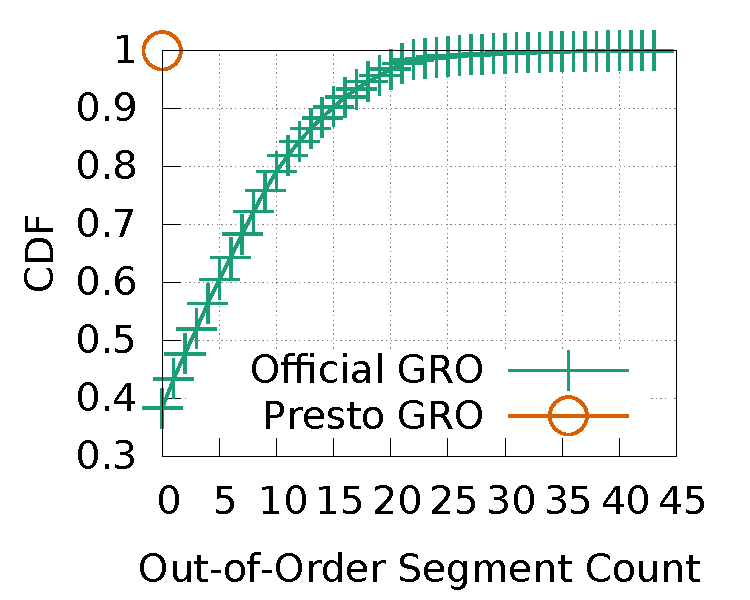
\includegraphics[width=\textwidth]{./figures/gro_effectiveness/metric1_seg_cdf_compare.pdf}
		\caption{}
		\label{gro_effectiveness_on_reordering}
	\end{subfigure}
        \begin{subfigure}[b]{0.225\textwidth}
                \centering
		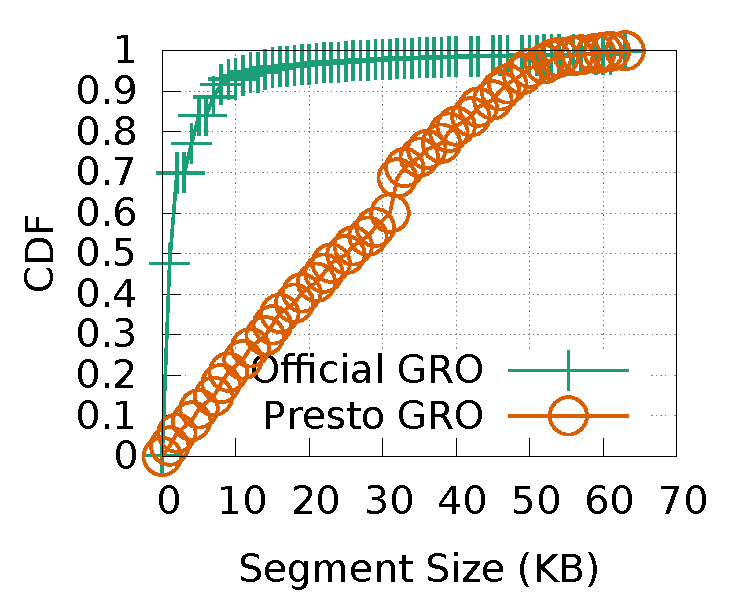
\includegraphics[width=\textwidth]{./figures/gro_effectiveness/metric1_pktsize_cdf_compare.pdf}
        	\caption{}
		\label{gro_effectiveness_on_pktsize}
	\end{subfigure}
	\caption{(a) Illustration of the modified GRO's effectiveness on masking reordering. 
		%We use the number of  segments from other chunks
                %between the first segment and last segment of each chunk
                %seen by TCP to measure the extent of packet reordering
		(b) In case of massive packet reordering, official GRO cannot merge packets effectively such that lots of small
                packets are processed by TCP which poses great processing overhead for CPU.}
	\label{gro_effectiveness}
\end{figure}

\tightparagraph{Presto's GRO Combats Reordering}
To examine Presto's ability to handle packet reordering, we perform a simple experiment
on topology shown in Figure~\ref{micro_congestion_topology}.
%we compare the extent of TCP reordering, TCP segment size distribution, throughput and receiver side CPU usage 
%using official GRO and Presto GRO. 
Here two servers attached to leaf switch L1 
send traffic to their own receivers attached to leaf switch L2
by spreading 64KB flowcells over the two network paths. 
%Because these two flows share the same two paths 
%so packet reordering can happen at the receiver side.
This setup can cause reordering for each flow, so 
we compare Presto's GRO to
an unmodified GRO, denoted "Official GRO". 
The amount of reordering exposed to TCP is presented in Figure~\ref{gro_effectiveness_on_reordering}.
To quantify packet reordering, we show a CDF of the {\em out-of-order segment count}:~\ie{},
the number of segments from other flowcells between the first packet and last packet of each flowcell. A value of zero
means there is no reordering and larger values mean more reordering. The figure shows Presto's GRO can completely mask reordering
while official GRO incurs significant reordering. As shown in Section~\ref{sec:background}, reordering can
also cause smaller segments to be pushed up the networking stack, causing significant processing overhead.
Figure~\ref{gro_effectiveness_on_pktsize} shows the received TCP segment size distribution.  Presto's GRO
pushes up large segments, while the official GRO pushes up many small segments.
The average TCP throughputs in official GRO and Presto GRO are 4.6Gbps (with 86\% CPU utilization) and 
9.3Gbps (with 69\% CPU utilization), respectively. Despite the fact that official GRO only obtains 
about half the throughput of Presto's GRO, it still incurs more than 24\% higher CPU overhead. 
Therefore, an effective scheme must deal with both reordering and small segment overhead.
%\eric{interesting that stride on big testbed w/ official GRO had same numbers: 4.6 Gbps and similar overhead}

\begin{figure}[t]
        \centering
  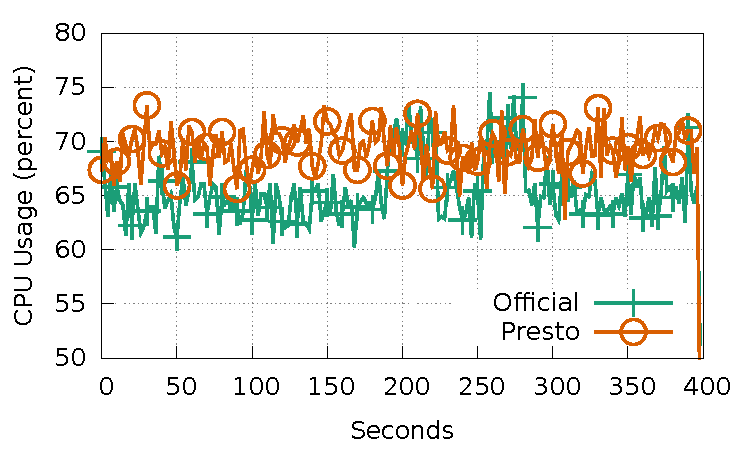
\includegraphics[width=0.45\textwidth]{./figures/mornitor_cpu/macro_compare_cpu_usage.pdf}
        \caption{Presto incurs 6\% CPU overhead on average.}
        \label{micro_compare_cpu}
\end{figure}

\tightparagraph{Presto Imposes Limited CPU Overhead}
We investigate Presto's CPU usage by
running the stride workload on a 2-tier Clos network as shown in Figure~\ref{macro_evaluation_topology}. 
For comparison, official GRO is run with the stride workload using a non-blocking switch (so there
is no reordering). Note both official GRO and Presto GRO can achieve 9.3Gbps.  
The receiver CPU usage is sampled every 2 seconds over a 400 second interval, and
the time-series is shown in Figure~\ref{micro_compare_cpu}. 
%implying that the network utilization is 93% in both cases. 
On average, Presto GRO only increases CPU usage by 6\% compared with the official GRO. 
The minimal CPU overhead comes from Presto's careful design and implementation. 
At the sender, Presto needs just two {\tt memcpy} operations (1 for shadow MAC rewriting, 1 for flowcell ID encoding). 
At the receiver, Presto needs one {\tt memcpy} to rewrite the shadow MAC back to the real MAC and
also incurs slight overhead because multiple segments are now kept per flow. The overhead
of the latter is reduced because these segments are largely kept in reverse sorted order, which means {\tt merge}
on an incoming packet is usually $\mathcal{O}(1)$. The insertion sort is done at the beginning of each {\tt flush} event over a small
number of mostly in-order segments, which easily amortizes overhead because it is called infrequently compared to {\tt merge}.

%%%%%scalability test figures %%%%
\begin{figure}[t]
        \centering
  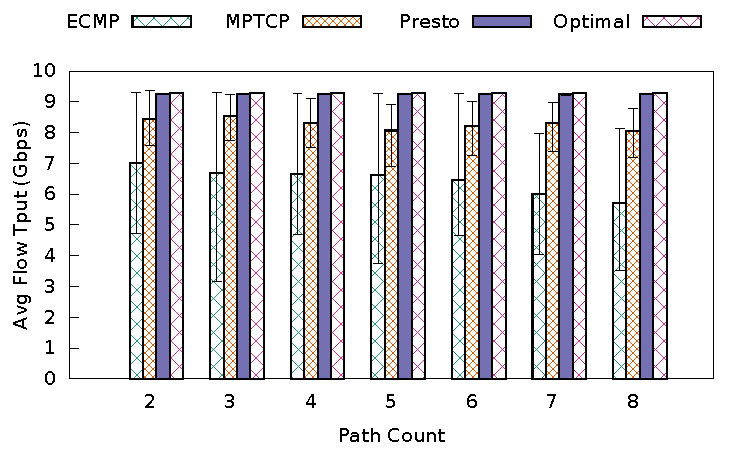
\includegraphics[width=0.45\textwidth]{./figures/scalability_test/scalability_compare_tput_witherrbar.pdf}
        \caption{Throughput comparison in scalability benchmark. We denote the non-blocking case as Optimal. 
		} 
        \label{micro_scalability_test_tput}
\end{figure}

%merged with scalability loss rate
\iffalse
\begin{figure}[ht]
        \centering
  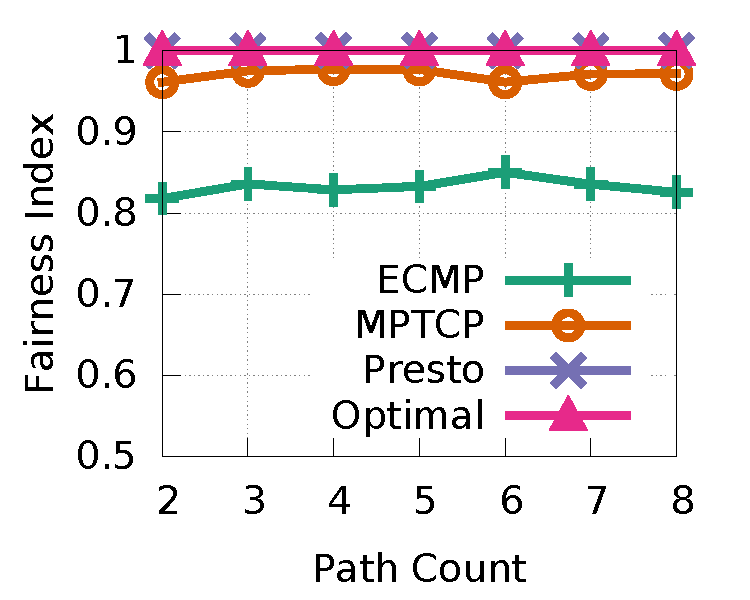
\includegraphics[width=0.45\textwidth]{./figures/scalability_test/scalability_compare_fairness.pdf}
        \caption{Micro benckmark 2 - scalability test. 
		We increase the number of spine switches (i.e., the number of intermediate paths)
                and set the number of flows (host pairs) equal to the number of available paths. 
		Fairness comparison. 20 runs each with each run lasting for 10 seconds.
		Optimal means running TCP on a non-blocking network}
        \label{micro_scalability_test_fairness}
\end{figure}
\fi

\begin{figure}[t]
        \centering
  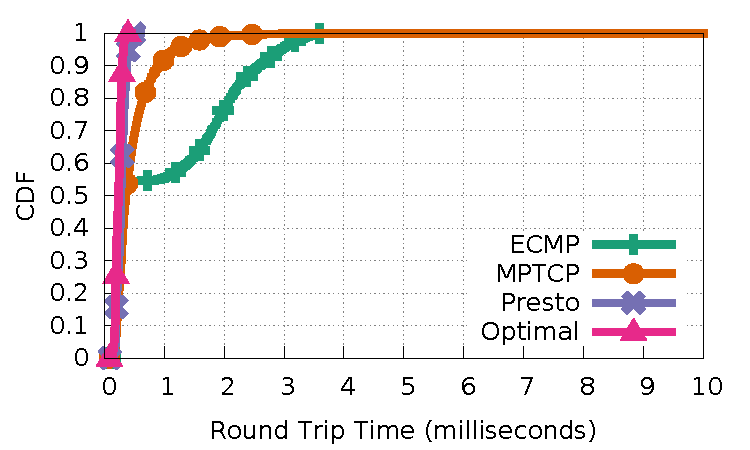
\includegraphics[width=0.45\textwidth]{./figures/scalability_test/scalability_compare_latency.pdf}
        \caption{Round trip time comparison in scalability benchmark. 
		%We increase the number of spine switches (i.e., the number of intermediate paths)
                %and set the number of flows (host pairs) equal to the number of available paths. 
		}
        \label{micro_scalability_test_latency}
\end{figure}


\begin{figure}[t]
        \centering
	\centering
        \begin{subfigure}[b]{0.225\textwidth}
                \centering
		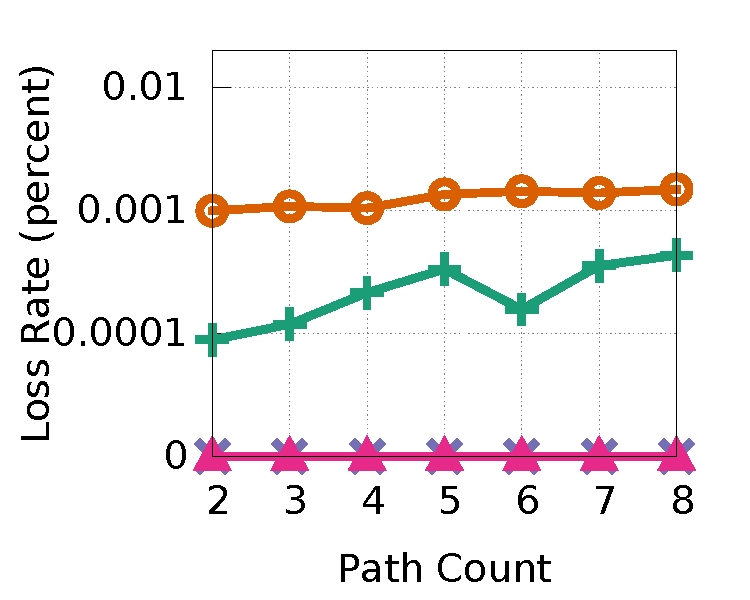
\includegraphics[width=\textwidth]{./figures/scalability_test/scalability_compare_loss.pdf}
		\caption{}
		\label{micro_scalability_test_loss}
        \end{subfigure}
        \begin{subfigure}[b]{0.225\textwidth}
  		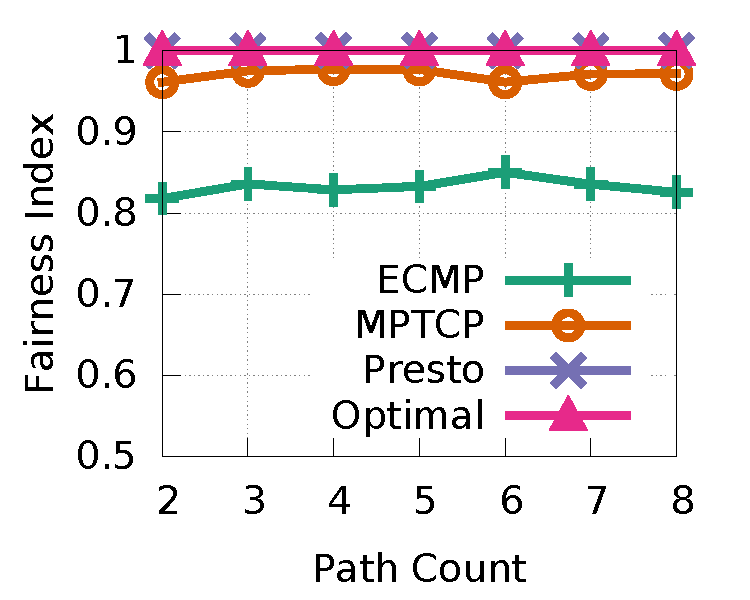
\includegraphics[width=\textwidth]{./figures/scalability_test/scalability_compare_fairness.pdf}
        	\caption{}
        	\label{micro_scalability_test_fairness}
	\end{subfigure}
	\caption{(a) Loss rate and (b) Fairness index comparison in scalability benchmark.}
\end{figure}

\tightparagraph{Presto Scales to Multiple Paths}
We analyze Presto's ability to scale in the number of paths by
setting the number of flows (host pairs) equal to the number of available paths in the topology shown in 
Figure~\ref{micro_scalability_topology}. The number of paths is varied from 2 to 8, and 
Presto always load-balances over all available paths.
Figure~\ref{micro_scalability_test_tput} shows Presto's throughput closely tracks Optimal. 
ECMP (and MPTCP) suffer from lower throughput when flows (or subflows) are
hashed to the same path. Hashing on the same path leads to congestion and thus increased latency, as shown in Figure~\ref{micro_scalability_test_latency}.
Because this topology is non-blocking and Presto load-balances in a near optimal fashion, Presto's latency
is near Optimal. Packet drop rates are presented in Figure~\ref{micro_scalability_test_loss} and show
Presto and Optimal have no loss. MPTCP has higher loss because of its bursty nature~\cite{conga}
and its aggression in the face of loss: when a single loss occurs, only
one subflow reduces its rate. The other schemes are more conservative because a single loss reduces the rate of the whole flow.
Finally, Figure~\ref{micro_scalability_test_fairness} shows Presto, Optimal and MPTCP
achieve almost perfect fairness.
%The underlying reason is that MPTCP makes traffic more bursty~\cite{conga}.


%%%congestion test figures %%%%
\begin{figure}[t]
        \centering
  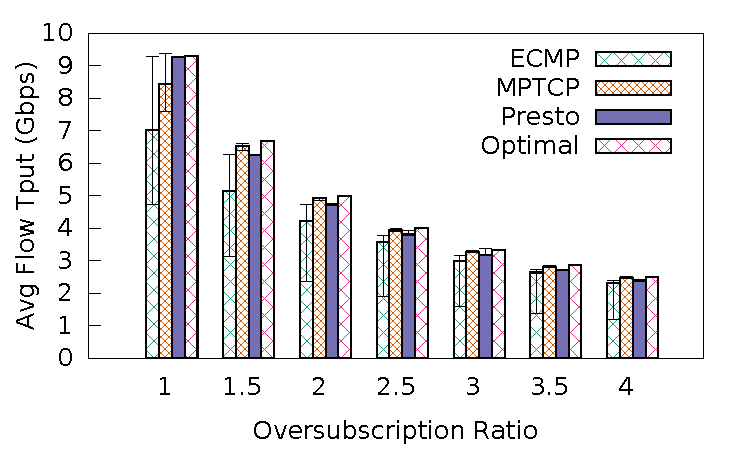
\includegraphics[width=0.45\textwidth]{./figures/congestion_test/congestion_compare_tput_witherrbar.pdf}
        \caption{Throughput comparison in oversubscription benchmark.}
        \label{micro_congestion_test_tput}
\end{figure}


\begin{figure}[t]
        \centering
  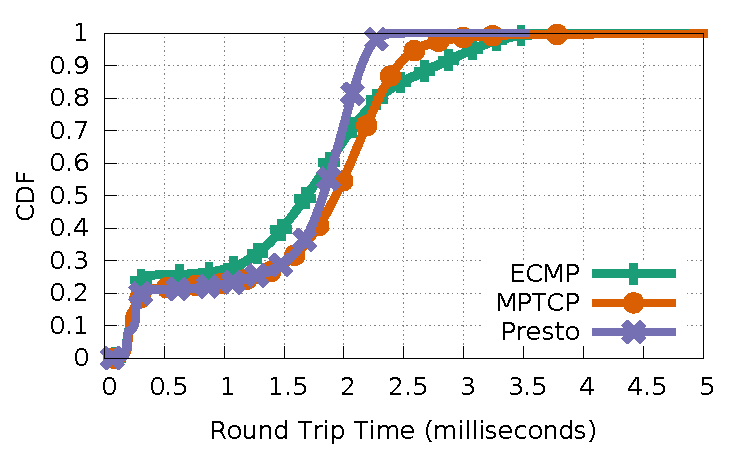
\includegraphics[width=0.45\textwidth]{./figures/congestion_test/congestion_compare_latency.pdf}
        \caption{Round trip time comparison in oversubscription benchmark.
		}
        \label{micro_congestion_test_latency}
\end{figure}



\begin{figure}[t]
        \centering
	\centering
        \begin{subfigure}[b]{0.225\textwidth}
                \centering
		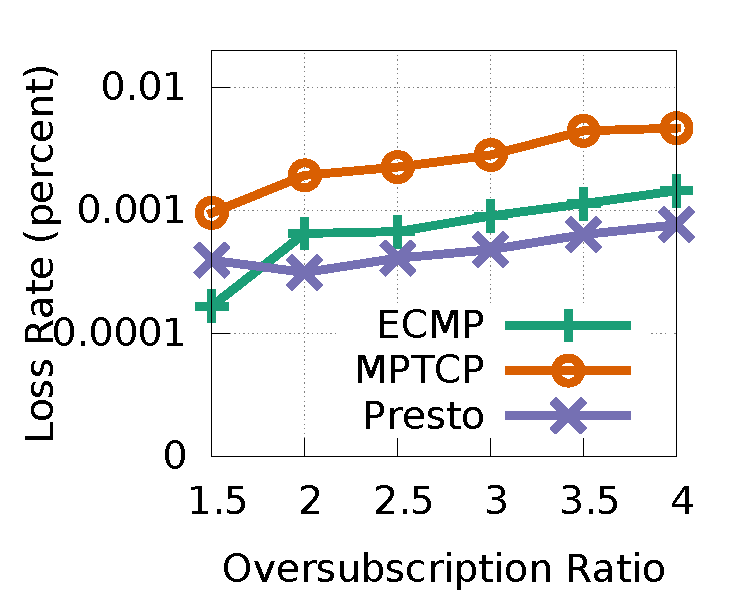
\includegraphics[width=\textwidth]{./figures/congestion_test/congestion_compare_loss.pdf}
		\caption{}
		\label{micro_congestion_test_loss}
	\end{subfigure}
	\begin{subfigure}[b]{0.225\textwidth}
		\centering
  		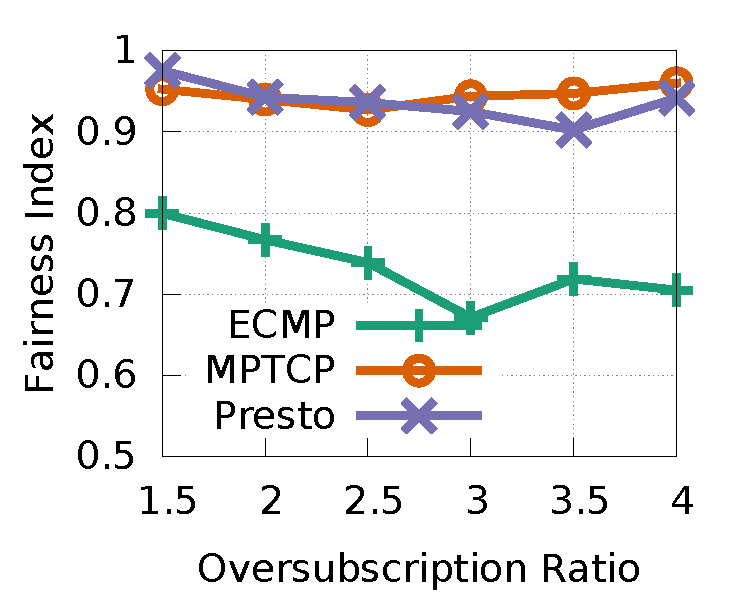
\includegraphics[width=\textwidth]{./figures/congestion_test/congestion_compare_fairness.pdf}
		\caption{}
        \label{micro_congestion_test_fairness}
	\end{subfigure}
	\caption{(a) Loss rate and (b) Fairness index comparison in oversubscription benchmark.}
\end{figure}

\tightparagraph{Presto Handles Congestion Gracefully}
Presto's ability to handle congestion is analyzed by fixing 
the number of spine and leaf switches to 2 and varying
the number of flows (host pairs) from 2 to 8, as shown
in Figure~\ref{micro_congestion_topology}. 
Each flow sends as much as possible, which leads to the network
being oversubscribed by a ratio of 1 (two flows) to 4 (eight flows).
Figure~\ref{micro_congestion_test_tput} shows all schemes track Optimal in highly
oversubscribed environments. ECMP
does poorly under moderate congestion because the limited number of flows can be hashed to the same path.
Presto does no worse in terms of latency (Figure~\ref{micro_congestion_test_latency}) and loss (Figure~\ref{micro_congestion_test_loss}).
The long tail latency for MPTCP is caused by its higher loss rates.
Both Presto and MPTCP have greatly improved fairness compared with ECMP (Figure~\ref{micro_congestion_test_fairness}).

\begin{figure}[t]
        \centering
  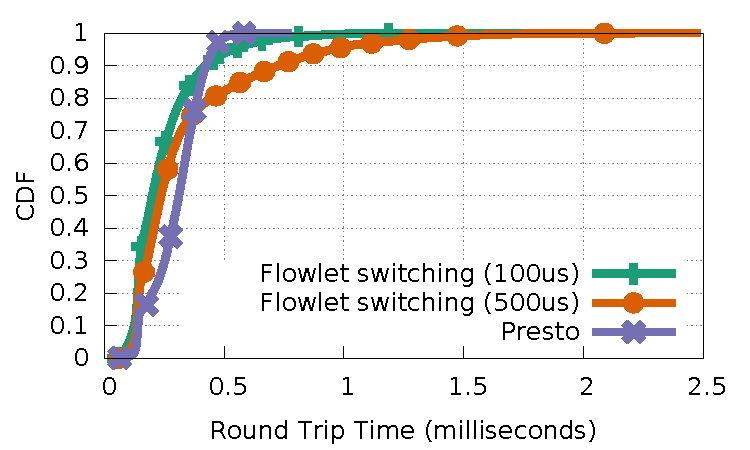
\includegraphics[width=0.45\textwidth]{./figures/flowlets/flowlet_switching/flowlet_presto_compare_sockperf.pdf}
        \caption{Round trip time comparison of Flowlet switching~\cite{flowlet,conga} and Presto in Stride workload. 
		The throughputs of Flowlet switching with 100 $\mu\text{s}$ gap, 500 $\mu\text{s}$ gap and Presto 
		are 4.3Gbps, 7.6Gbps and 9.3Gbps respectively. }
        \label{micro_flowlet_rtt_compare}
\end{figure}


\tightparagraph{Comparison to Flowlet Switching}
We implemented a flowlet load-balancing scheme in OVS that detects
inactivity gaps and then schedules flowlets over disjoint paths in a round robin fashion
(Presto does this over flowcells instead of flowlets).
The receiver for flowlets uses official GRO.
Presto is compared to 500 $\mu$s and 100 $\mu$s inactivity timers in
the stride workload on the 2-tier Clos network (Figure~\ref{macro_evaluation_topology}).
The throughput of the schemes are 9.3 Gbps (Presto), 7.6 Gbps (500 $\mu$s), and 4.3 Gbps (100 $\mu$s).
%Switching flowlets on very small timescales, such as 100$\mu$s, provides opportunities to create many flowlets.
%The largest flowlet is only 0.20\% (XX) of the total network traffic, which corresponds to about 5-9 MB in our runs.
%And while small flowlets create an even distribution
%of traffic over the network, significant strain is put on the TCP connection due to packet reordering. 
Analysis of the 100 $\mu$s
network traces show 13\%-29\% packets in the connection are reordered, which means 100 $\mu$s is not enough
time to allow packets to arrive in-order at the destination and thus throughput is severely impacted. Switching flowlets with 500 $\mu$s prevents
most reordering (only 0.03\%-0.5\% packets are reordered), but creates very large flowlets (see Figure~\ref{micro_flowlet_size}). This means
flowlets can still suffer from collisions, which can hurt throughput (note: while not shown here, 500 $\mu$s outperforms ECMP by over 40\%).
Figure~\ref{micro_flowlet_rtt_compare} shows the
latencies. Flowlet 100 $\mu$s has low throughput and hence lower latencies. However, since
its load balancing isn't perfect, it can still cause increased congestion in the tail. Flowlet 500 $\mu$s
also has larger tail latencies because of more pronounced flowlet collisions. As compared to the flowlet
schemes, Presto decreases 99.9$^{th}$ percentile latency by 2x-3.6x.
%Presto, by enforcing small flowlet sizes and explicitly accounting for reordering on the receiver, can obtain near
%line rate throughput with minimal tail latencies. 



%%%%presto 2 mods (ecmp and shaodw MAC) compare
\begin{figure}[t]
        \centering
  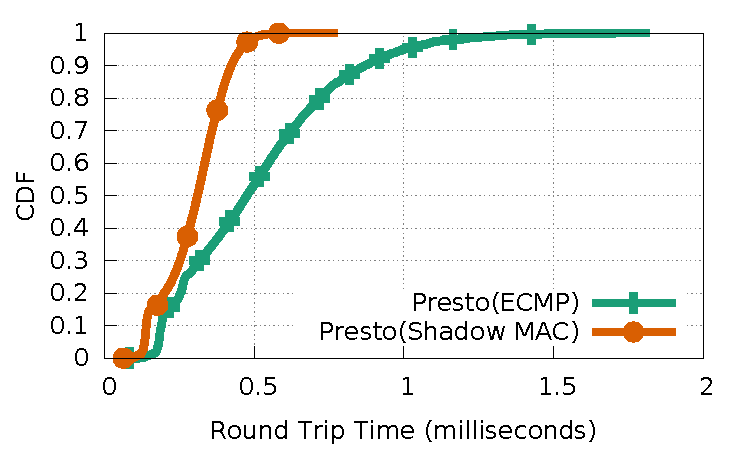
\includegraphics[width=0.45\textwidth]{./figures/presto_compare_2modes/presto_compare_2mods.pdf}
        \caption{Round trip time comparison between Presto + shadow MAC and Presto + ECMP.
		%Compare Presto 2 modes' (Presto over ECMP and Presto over Shadow MAC) performance.
                %Simple 2-tier Clos network with 4 senders and 4 receivers, 4 paths between any host pair.
                %10 seconds per run, 20 runs. Use {\tt nuttcp} to measure throughput. Use {\tt sockperf}
                %to measure latency (RTT).
                %In Presto+ECMP, the average throughput is 7.9 (8.7 if trade latency for tput)
                %Gbps while in Presto+Shadow MAC, the
                %average throughput is 9.3Gbps 
		}
        \label{micro_presto_2mods}
\end{figure}

\tightparagraph{Comparison to Local, Per-Hop Load Balancing}
Presto sends flowcells in a round robin fashion over pre-configured end-to-end paths. An alternative is to
have ECMP hash on flowcell ID and thus provide per-hop load balancing. 
%One way to implement Presto + ECMP is to let vSwitch copy real TCP source port into a pre-allocated TCP option field 
%(\todo{this requires TCP stack allocates the new TCP option before sending to vSwitch}) and 
%encode chunk ID into TCP source port field. Because chunk ID is incremental, ECMP randomly maps chunks into multiple paths. 
We compare Presto + shadow MAC with Presto + ECMP using a stride workload on our testbed. 
Presto + shadow MAC's average throughput is 9.3Gbps while Presto + ECMP's is 8.9Gbps.
The round trip time CDF is shown in Figure~\ref{micro_presto_2mods}. 
Presto + shadow MAC gives better latency performance compared with Presto + ECMP. 
The performance difference comes from the fact that Presto + shadow MAC provides 
better fine-grained flowcell load balancing because 
randomization in per-hop multipathing can lead to corner cases where
a large fraction of flowcells get sent to the same link over a small timescale by multiple flows. This transient congestion
can lead to increased buffer occupancy and higher delays in the network.
